\documentclass[12pt, a4paper, oneside]{ctexart}
\usepackage{amsmath, amsthm, amssymb, bm, color, graphicx, geometry, mathrsfs,extarrows, braket, booktabs, array}
\usepackage[colorlinks,linkcolor=red,anchorcolor=blue,citecolor=blue,urlcolor=blue,menucolor=black]{hyperref}
%%%% 设置中文字体 %%%%
\setCJKmainfont{方正新书宋_GBK.ttf}[BoldFont=方正小标宋_GBK, ItalicFont=方正楷体_GBK]
%%%% 设置英文字体 %%%%
\setmainfont{Times New Roman}
\setsansfont{Calibri}
\setmonofont{Consolas}

\linespread{1.4}
%\geometry{left=2.54cm,right=2.54cm,top=3.18cm,bottom=3.18cm}
\geometry{left=1.84cm,right=1.84cm,top=2.18cm,bottom=2.18cm}
\newcounter{problem}  % 问题序号计数器
\newenvironment{problem}[1][]{\stepcounter{problem}\par\noindent\textbf{题目\arabic{problem}. #1}}{\smallskip\par}
\newenvironment{solution}[1][]{\par\noindent\textbf{#1解答. }}{\smallskip\par}  % 可带一个参数表示题号\begin{solution}{题号}
\newenvironment{note}{\par\noindent\textbf{注记. }}{\smallskip\par}

%%%% 图片相对路径 %%%%
\graphicspath{{figure/}} % 当前目录下的figure文件夹, {../figure/}则是父目录的figure文件夹
\setlength{\abovecaptionskip}{-0.2cm}  % 缩紧图片标题与图片之间的距离
\setlength{\belowcaptionskip}{0pt} 

\everymath{\displaystyle} % 默认全部行间公式
\DeclareMathOperator*\uplim{\overline{lim}} % 定义上极限 \uplim_{}
\DeclareMathOperator*\lowlim{\underline{lim}} % 定义下极限 \lowlim_{}
\DeclareMathOperator*{\argmax}{arg\,max}  % \argmin
\DeclareMathOperator*{\argmin}{arg\,min}  % \argmax
\let\leq=\leqslant % 将全部leq变为leqslant
\let\geq=\geqslant % geq同理
\DeclareRobustCommand{\rchi}{{\mathpalette\irchi\relax}}
\newcommand{\irchi}[2]{\raisebox{\depth}{$#1\chi$}} % 使用\rchi将\chi居中

%%%% 一些宏定义 %%%%
\def\bd{\boldsymbol}        % 加粗(向量) boldsymbol
\def\disp{\displaystyle}    % 使用行间公式 displaystyle(默认)
\def\tsty{\textstyle}       % 使用行内公式 textstyle
\def\sign{\text{sign}}      % sign function
\def\wtd{\widetilde}        % 宽波浪线 widetilde
\def\R{\mathbb{R}}          % Real number
\def\N{\mathbb{N}}          % Natural number
\def\Z{\mathbb{Z}}          % Integer number
\def\Q{\mathbb{Q}}          % Rational number
\def\C{\mathbb{C}}          % Complex number
\def\N{\mathbb{N}}          % Natural number
\def\Z{\mathbb{Z}}          % Integer number
\def\E{\mathbb{E}}          % Exception
\def\var{\text{Var}}        % Variance
\def\cov{\text{Cov}}        % Coefficient of Variation
\def\bias{\text{bias}}      % bias
\def\d{\mathrm{d}}          % differential operator
\def\e{\mathrm{e}}          % Euler's number
\def\i{\mathrm{i}}          % imaginary number
\def\re{\mathrm{Re}}        % Real part
\def\im{\mathrm{Im}}        % Imaginary part
\def\res{\mathrm{Res}}      % Residue
\def\L{\mathcal{L}}         % Loss function
\def\wdh{\widehat}          % 宽帽子 widehat
\def\ol{\overline}          % 上横线 overline
\def\ul{\underline}         % 下横线 underline
\def\add{\vspace{1ex}}      % 增加行间距
\def\del{\vspace{-1.5ex}}   % 减少行间距

%%%% 定理类环境的定义 %%%%
\newtheorem{theorem}{定理}

%%%% 基本信息 %%%%
\newcommand{\RQ}{\today} % 日期
\newcommand{\km}{数理统计} % 科目
\newcommand{\bj}{强基数学002} % 班级
\newcommand{\xm}{吴天阳} % 姓名
\newcommand{\xh}{2204210460} % 学号
\newcommand{\id}{50} % 序号

\begin{document}

%\pagestyle{empty}
\pagestyle{plain}
\vspace*{-15ex}
\centerline{\begin{tabular}{*6{c}}
    \parbox[t]{0.25\linewidth}{\begin{center}\textbf{日期}\\ \large \textcolor{blue}{\RQ}\end{center}} 
    & \parbox[t]{0.2\linewidth}{\begin{center}\textbf{科目}\\ \large \textcolor{blue}{\km}\end{center}}
    & \parbox[t]{0.2\linewidth}{\begin{center}\textbf{班级}\\ \large \textcolor{blue}{\bj}\end{center}}
    & \parbox[t]{0.1\linewidth}{\begin{center}\textbf{姓名}\\ \large \textcolor{blue}{\xm}\end{center}}
    & \parbox[t]{0.15\linewidth}{\begin{center}\textbf{学号}\\ \large \textcolor{blue}{\xh}\end{center}}
    & \parbox[t]{0.1\linewidth}{\begin{center}\textbf{序号}\\ \large \textcolor{blue}{\id}\end{center}}
     \\ \hline
\end{tabular}}
\begin{center}
    \zihao{3}\textbf{第六次作业}
\end{center}\vspace{-0.2cm}
% 正文部分
\begin{problem}[(1)]
    令$X$是来自分布$f(x;\theta) = \theta x^{\theta-1}I_{(0,1)}(x),\ \theta > 0$.

    (a) 求一个枢轴量,并且使用它求出关于$\theta$的一个置信区间估计.

    (b) 令$Y = -1/\log X$,则$(Y/2,Y)$关于$\theta$的置信区间,求出关于该区间的置信系数,并且找到一个关于$\theta$更优的置信区间.
\end{problem}
\begin{solution}
    (a) 由于$X$分布函数$F(x) = \int_0^x\theta t^{\theta-1}\,\d t=x^{\theta},\ (0<x<1)$. 由于$F(X)\sim I(0,1)$,则$-\log F(X) \sim\Gamma(1,1)\Rightarrow -2\log F(X)\sim \rchi^2(2)$. 设$q_1,q_2\in(0,\infty),\ q_1<q_2$,满足
    \begin{equation*}
        \gamma = P(q_1 < -2\log F(x) < q_2) = P(q_1 < -2\theta\log X < q_2) = P\left(\frac{q_1}{-2\log X} < \theta < \frac{q_2}{-2\log X}\right)
    \end{equation*}

    $q_1,q_2$取等尾概率$q_1 = \rchi^2_{\frac{1-\gamma}{2}}(2),\ q_2 = \rchi^2_{\frac{1+\gamma}{2}}(2)$,则$\theta$的一个系数为$\gamma$的置信区间为
    \begin{equation*}
        \left(\frac{\rchi^2_{\frac{1-\gamma}{2}}(2)}{-2\log X} ,\frac{\rchi^2_{\frac{1+\gamma}{2}}(2)}{-2\log X}\right)
    \end{equation*}

    (b) 由于$(Y/2,Y)$是$\theta$的一个置信区间,则
    \begin{equation*}
        P(Y/2<\theta<Y) = P(1/2<\theta/Y<1) = P(1/2<-\theta\log X<1)
    \end{equation*}
    由于$-\theta\log X\sim\Gamma(1,1)$,于是$P(Y/2<\theta<Y) = \int_{\frac{1}{2}}^1\e^{-x} = \e^{-\frac{1}{2}}-\e^{-1}$,于是该区间的置信系数$\gamma = \e^{-\frac{1}{2}}-\e^{-1}$. 设$q_1,q_2\in[0,\infty),\ q_1<q_2$满足
    \begin{equation*}
        \gamma = P(q_1 < -\theta\log X<q_2) = P\left(\frac{q_1}{-\log X} < \theta < \frac{q_2}{-\log X}\right)
    \end{equation*}
    则期望区间长度$l = \E\left[\frac{q_1}{\log X} - \frac{q_2}{\log X}\right] = \E\left[\frac{1}{\log X}\right](q_1-q_2)$,\add 由于$\E\left[\frac{1}{\log X}\right] < 0$,则极小化$l$$\iff$极大化$q_1-q_2$,转化为求解极大化问题
    \begin{align*}
        \max&\quad z=q_1-q_2,\\
        s.t.&\quad \int_{q_1}^{q_2}\e^{-x}\,\d x = \e^{-q_1}-\e^{-q_2} = \gamma,\\
        &\quad 0 \leq q_1 < q_2.
    \end{align*}
    于是$q_1 = -\log(\e^{-q_2}+\gamma)$,由于$q_1\geq0$代入得到$q_2 \geq -\log(1-\gamma)$且
    \begin{equation*}
        z = -\log(\e^{-q_2}+\gamma)-q_2,\ z' = \frac{-\gamma}{\e^{-q_2}+\gamma} < 0
    \end{equation*}
    则$z$关于$q_2$单调递减,于是$q_2 = -\log(1-\gamma)$时$z$有极大值,区间长度有极小值,对应的$q_1 = 0$,则更优的置信区间为
    \begin{equation*}
        \left(0,\frac{\log(1-\gamma)}{\log X}\right) = \left(0, \frac{\log(1+\e^{-1}-\e^{-\frac{1}{2}})}{\log X}\right)
    \end{equation*}
\end{solution}
\begin{problem}[(2)]
    令$X_1,\cdots, X_n$是来自$N(\theta,\theta),\ \theta>0$的随机样本. 求出一个枢轴量,并用它得到关于$\theta$的置信区间估计.
\end{problem}
\begin{solution}
    由于$\frac{\bar{X}-\theta}{\sqrt{\theta/n}}\sim N(0,1)$,$\frac{X_i-\theta}{\sqrt{\theta}}\sim N(0,1)$,于是$\sum_{i=1}^n\left(\frac{X_i-\bar{X}}{\sqrt{\theta}}\right)^2=\frac{(n-1)S^2}{\theta}\sim\rchi^2(n-1)$,于是
    \begin{equation*}
        \frac{\bar{X}-\theta}{\sqrt{\theta/n}}\cdot\frac{\sqrt{\theta(n-1)}}{\sqrt{(n-1)S^2}} = \sqrt{n}\frac{\bar{X}-\theta}{S}\sim t(n-1)
    \end{equation*}
    设$q_1,q_2\in \R,\ q_1<q_2$,满足
    \begin{equation*}
        \gamma = P(q_1 < \sqrt{n}\frac{\bar{X}-\theta}{S} < q_2) = P\left(\bar{X}-\frac{S}{\sqrt{n}}q_2< \theta <\bar{X}-\frac{S}{\sqrt{n}}q_1\right)
    \end{equation*}
    由于$t$分布为对称分布,则$q_2=-q_1 = t_{\frac{1+\gamma}{2}}(n-1)$是使得置信区间最小的上下限,则$\theta$的系数为$\gamma$的置信区间为
    \begin{equation*}
        \left(\bar{X}-\frac{S}{\sqrt{n}}t_{\frac{1+\gamma}{2}}(n-1), \bar{X}+\frac{S}{\sqrt{n}}t_{\frac{1+\gamma}{2}}(n-1)\right)
    \end{equation*}
\end{solution}
\begin{problem}[(5)]
    令$X_1,\cdots,X_n$是来自$f(x;\theta) = \theta\e^{-\theta x}I_{(0,\infty)}(x)$的随机样本.

    (a) 求解关于总体均值的$100\gamma$置信度区间.

    (b) 求解关于总体方差的$100\gamma$置信度区间.

    (c) 求解上述两个区间同时覆盖真实均值和方差的概率.

    (d) 求解关于$\e^{-\theta} = P(X>1)$的置信区间估计.

    (e) 求出仅与$Y_1$相关的枢轴量,并且使用它求出关于$\theta$的置信区间估计.
\end{problem}
\begin{solution}
    (a) 总体均值为$\E(\bar{X}) = \E(X) = 1/\theta$. 由于$\theta$为尺度参数,$\theta X\sim \gamma(1,1)$,则$\theta\sum_{i=1}^nX_i\sim \Gamma(n,1)\Rightarrow 2\theta\sum_{i=1}^nX_i\sim\rchi^2(2n)$. 设$q_1,q_2\in[0,\infty),\ q_1<q_2$,满足
    \begin{equation*}
        \gamma = P(q_1 < 2\theta\sum_{i=1}^nX_i < q_2) = P\left(\frac{2n\bar{X}}{q_2}<\frac{1}{\theta}<\frac{2n\bar{X}}{q_1}\right)
    \end{equation*}
    对$q_1,q_2$取等尾概率得$q_1 = \rchi^2_{\frac{1-\gamma}{2}}(2n),\ q_2=\rchi^2_{\frac{1+\gamma}{2}}(2n)$,于是总体均值$1/\theta$的置信度为$100\gamma$的区间为
    \begin{equation*}
        \left(\frac{2n\bar{X}}{\rchi^2_{\frac{1+\gamma}{2}}(2n)}, \frac{2n\bar{X}}{\rchi^2_{\frac{1-\gamma}{2}}(2n)}\right)
    \end{equation*}

    (b) 由于总体方差为$\var(X) = 1/\theta^2$,且$P(q_1'<1/\theta<q_2') = P(q_1'^2<1/\theta<q_2'^2)$,由(a)可得,总体方差$1/\theta^2$的置信度为$100\gamma$的区间为
    \begin{equation*}
        \left(\left[\frac{2n\bar{X}}{\rchi^2_{\frac{1+\gamma}{2}}(2n)}\right]^2, \left[\frac{2n\bar{X}}{\rchi^2_{\frac{1-\gamma}{2}}(2n)}\right]^2\right)
    \end{equation*}

    (c) 由于(b)是由(a)直接推出的,所以同时包含住真实均值和方差的概率为$\gamma$.\add

    (d) 由(a)可知,$P\left(\frac{q_1}{2n\bar{X}} < \theta < \frac{q_2}{2n\bar{X}}\right) = P\left(\exp\left\{-\frac{q_2}{2n\bar{X}}\right\}<\e^{-\theta}<\exp\left\{-\frac{q_1}{2n\bar{X}}\right\}\right) = \lambda$,\add 于是$\e^{-\theta}$的系数为$\lambda$的置信区间为
    \begin{equation*}
        \left(\exp\left\{-\frac{q_2}{2n\bar{X}}\right\},\exp\left\{-\frac{q_1}{2n\bar{X}}\right\}\right)
    \end{equation*}

    (e) 由于$f_{Y_1}(y) = nf_X(y)(1-F_X(y))^{n-1} = n\theta\e^{-n\theta y}\sim \Gamma(1,n\theta)$,令$Z = \theta Y_1$,则$f_Z(z) = f_{Y_1}(z/\theta)/\theta = n\e^{-nz}\sim \Gamma(1,n)$. 设$q_1,q_2\in [0,\infty),\ q_1 < q_2$,满足
    \begin{equation*}
        1-\alpha = P(q_1 < \theta Y_1 < q_2) = P\left(\frac{q_1}{Y_1} < \theta < \frac{q_2}{Y_1}\right)
    \end{equation*}
    于是期望区间长度为\add $l = \E\left[\frac{q_2}{Y_1}-\frac{q_1}{Y_1}\right] = \E\left[\frac{1}{Y_1}\right](q_2-q_1)$,由于$\E\left[\frac{1}{Y_1}\right]>0$,于是最小化$l\iff$最小化$q_2-q_1$,转化为求解极小化问题
    \begin{align*}
        \min&\quad z=q_2-q_1,\\
        s.t.&\quad \int_{q_1}^{q_2}n\e^{-nz}\,\d z = \e^{-nq_1}-\e^{-nq_2} = 1-\alpha\\
        &\quad 0 \leq q_1 < q_2.
    \end{align*}
    则$q_1 = -\frac{1}{n}\log(1-\alpha + \e^{-nq_2})$,由于$q_1 \geq 0$代入可得$q_2\geq -\frac{1}{n}\log \alpha$且
    \begin{equation*}
        z = q_1+\frac{1}{n}\log(1-\alpha+\e^{-nq_2}),\ f'(q_2)=1-\frac{\e^{-nq_2}}{1-\alpha+\e^{-nq_2}} > 0
    \end{equation*}
    则$z$关于$q_2$单调递增,当$q_2 = -\frac{1}{n}\log\alpha$时$z$有极小值,对应$q_1 = 0$,于是$\theta$的系数为$1-\alpha$的置信区间为
    \begin{equation*}
        \left(0,-\frac{\log\alpha}{nY_1}\right)
    \end{equation*}
\end{solution}
\begin{problem}[(18)]
    为了在正常耕作条件下测试两个新型杂交玉米品种,一家种子公司在Iowa选择了八个农场,并在每个农场的试验田里终止了两个新品种. 八个地点的产量为(换算为蒲式耳/英尺)\del
\renewcommand\arraystretch{0.8} % 设置表格高度为原来的0.8倍
\begin{table}[!htbp] % table标准
    \centering % 表格居中
    \begin{tabular}{p{3cm}<{\centering}p{1cm}<{\centering}p{1cm}<{\centering}p{1cm}<{\centering}p{1cm}<{\centering}p{1cm}<{\centering}p{1cm}<{\centering}p{1cm}<{\centering}p{1cm}<{\centering}} % 设置表格宽度
    %\begin{tabular}{cccc}
        Line A:&86&87&56&93&84&93&75&79\\
        Line B:&80&79&58&91&77&82&74&66\\
    \end{tabular}
\end{table}\del

假设假设两个收益率满足联合正态分布,求解两个品种平均收益率之差满足系数为$95$的置信区间.
\end{problem}
\begin{solution}
    \add 设品种$A,B$收益率对应的样本为$X_1,\cdots,X_8;\ Y_1,\cdots,Y_8$,则$(X_1,Y_1),\cdots,(X_8,Y_8)\overset{iid}{\sim}N\left(\left(\begin{matrix}
        \mu_1\\ \mu_2
    \end{matrix}\right),\left(\begin{matrix}
        \sigma_1^2&\rho\sigma_1\sigma_2\\
        \rho\sigma_1\sigma_2&\sigma_2^2
    \end{matrix}\right)\right)$,其中$\rho = \frac{\cov(X,Y)}{\sigma_1\sigma_2}$. \add 令$D_i = X_i-Y_i$则$D_i\sim N(\mu_1-\mu_2,\sigma_D^2)$,其中$\sigma_D^2 = \sigma_1^2+\sigma_2^2-2\rho\sigma_1\sigma_2$,则
    \begin{equation*}
        \frac{\bar{D}-(\mu_1-\mu_2)}{\sigma_D/\sqrt{n}}\sim N(0,1),\ \frac{\sum_{i=1}^n(D-\bar{D})^2}{\sigma_D^2} = \frac{(n-1)S_D^2}{\sigma_D^2}\sim \rchi^2(7)
    \end{equation*}
    于是$\frac{\bar{D}-(\mu_1-\mu_2)}{S_D/\sqrt{n}}\sim t(7)$,则置信度为95的区间为
    \begin{equation*}
        \left(\bar{D}-t_{0.975}(7)\frac{S_D}{\sqrt{8}}, \bar{D}+t_{0.975}(7)\frac{S_D}{\sqrt{8}}\right)
    \end{equation*}
    由于$D_i = 6,8,-2,2,7,11,1,13$,则$\bar{D} = 5.75,\ S_D \approx 5.12$,查表可得$t_{0.975}(7) \approx 2.365$,于是品种A与品种B收益率均值差的置信度为95的区间为$(1.469,10.031)$.
\end{solution}
\begin{problem}[(中文书3)]
    $0.50,1.25,0.80,2.00$是取自总体$X$的样本,已知$Y=\log X$服从正态分布$N(\mu,1)$.

    (1) 求$\mu$的置信水平为$95\%$的置信区间.

    (2) 求$X$的数学期望的置信水平为$95\%$的置信区间.
\end{problem}
\begin{solution}
    (1) 由于$Y_1,\cdots, Y_4\overset{iid}{\sim}N(\mu,1/4)$,则$\bar{Y}\sim(\mu,1/4)$,于是$\frac{\bar{Y}-\mu}{1/2}\sim N(0,1)$,设$q_1,q_2\in\R,\ q_1<q_2$满足
    \begin{equation*}
        0.95 = P(q_1 < 2(\bar{Y}-\mu) < q_2) = P\left(\bar{Y}-\frac{q_1}{2}<\mu<\bar{Y}-\frac{q_2}{2}\right)
    \end{equation*}
    由于正态分布是对称的,取$q_2=-q_1 = z_{0.975}\approx 1.96$时置信区间长度达到最小,且$\bar{Y} = \frac{1}{4}\log(\frac{1}{2}\cdot \frac{5}{4}\cdot\frac{4}{5}\cdot 2) = 0$,则$\mu$的置信水平为$95\%$的置信区间为$(-0.98, 0.98)$.

    (2) 由于
    \begin{align*}
        \E(X) =&\ \E(\e^Y) = \int_R\e^y\frac{1}{\sqrt{2\pi}}\e^{-\frac{(y-\mu)^2}{2}}\,\d y = \frac{1}{\sqrt{2\pi}}\int_R\e^{y+\mu}\e^{-\frac{y^2}{2}}\,\d y\\
        =&\ \frac{1}{\sqrt{2\pi}}\int_\R\e^{-\frac{(y-1)^2}{2}}\e^{\mu+\frac{1}{2}}\,\d y = \e^{\mu+\frac{1}{2}}
    \end{align*}
    由于$P(-0.98<\mu<0.98)\approx 0.95$,则$P(\e^{-0.98+0.5}<\e^{\mu+\frac{1}{2}} < \e^{0.98+0.5})\approx 0.95$,于是$\E(X)$的置信水平为$95\%$的置信区间为$(0.6188, 4.3929)$.
\end{solution}
\begin{problem}[(中文书5)]
    已知某种材料的抗压强度$X\sim N(\mu,\sigma^2)$,现随机地抽取$10$个试件进行抗压试验,测得数据如下:
    \begin{equation*}
        482\quad 493\quad  457\quad 471\quad 510\quad 446\quad 435\quad 418\quad 394\quad 469
    \end{equation*}

    (1) 求平均抗压强度$\mu$的置信水平为$95\%$的置信区间.

    (2) 若已知$\sigma=30$,求平均抗压强度$\mu$的置信水平为$95\%$的置信区间.

    (3) 求$\sigma$的置信水平为$95\%$的置信区间.
\end{problem}
\begin{solution}
    (1) 由于$\frac{\bar{X}-\mu}{\sigma/\sqrt{10}}\sim N(0,1)$,$\sum_{i=1}^{10}\left(\frac{X_i-\bar{X}}{\sigma}\right)^2=\frac{9S^2}{\sigma^2}\sim\rchi^2(9)$,则
    \begin{equation*}
        \frac{\bar{X}-\mu}{\sigma/\sqrt{10}}\frac{\sigma\sqrt{9}}{\sqrt{9}S} = \sqrt{10}\frac{\bar{X}-\mu}{S}\sim t(n-1)
    \end{equation*}
    设$q_1,q_2\in\R,\ q_1<q_2$满足
    \begin{equation*}
        \gamma = P\left(q_1 < \sqrt{10}\frac{\bar{X}-\mu}{S}<q_2\right) = P\left(\bar{X}-\frac{S}{\sqrt{10}}q_2<\mu<\bar{X}-\frac{S}{\sqrt{10}}q_1\right)
    \end{equation*}
    由于$t$为对称分布,取$q_2=-q_1 = t_{0.975}(9)\approx 2.365$,$\bar{X} = 457.5,\ S = \sqrt{\frac{1}{9}\sum_{i=1}^{10}(x_i-\bar{X})^2} \approx 35.2176$,则$\mu$的置信水平为$95\%$的置信区间为
    \begin{equation*}
        \left(\bar{X}-\frac{S}{\sqrt{10}}t_{0.975}(9),\bar{X}+\frac{S}{\sqrt{10}}t_{0.975}(9)\right) = (431.1615, 483.8385)
    \end{equation*}

    (2). 由于$\frac{\bar{X}-\mu}{30/\sqrt{10}}\sim N(0,1)$,设$q_1,q_2\in\R,\ q_1<q_2$满足
    \begin{equation*}
        \gamma = P\left(q_1<\frac{\bar{X}-\mu}{30/\sqrt{10}}<q_2\right)  = P\left(\bar{X}-\frac{30}{\sqrt{10}}q_2<\mu<\bar{X}-\frac{30}{\sqrt{10}}q_1\right)
    \end{equation*}
    由于$N(0,1)$为对称分布,取$q_2=-q_1 = z_{0.975}\approx 1.96$,$\mu$的置信水平为$95\%$的置信区间为
    \begin{equation*}
        \left(\bar{X}-\frac{30}{\sqrt{10}}z_{0.975}<\mu<\bar{X}+\frac{30}{\sqrt{10}}z_{0.975}\right) = (438.9058, 476, 0.942)
    \end{equation*}

    (3). 由于$\frac{X_i-\mu}{\sigma}\sim  N(0,1)$且$\sum_{i=1}^{10}\left(\frac{X_i-\bar{X}}{\sigma}\right)^2 = \frac{9S^2}{\sigma^2} \sim \rchi^2(9)$. 设$q_1,q_2\in[0,\infty),\ q_1 < q_2$满足
    \begin{equation*}
        \gamma = P\left(q_1<\frac{9S^2}{\sigma^2}<q_2\right) = P\left(\frac{3S}{\sqrt{q_2}}<\sigma<\frac{3S}{\sqrt{q_1}}\right)
    \end{equation*}
    由于$\chi^2$不是对称分布,考虑等尾分布:$q_1=\rchi^2_{0.025}(9)\approx 2.7,\ q_2=\rchi^2_{0.975}(9)\approx 19.023,\ S \approx 35.2176$,于是$\sigma$的置信水平为$95\%$的置信区间为
    \begin{equation*}
        \left(\frac{3S}{\sqrt{\rchi^2_{0.975}(9)}},\frac{3S}{\sqrt{\rchi^2_{0.025}(9)}}\right) = (24.2237, 64.2982)
    \end{equation*}
\end{solution}
\begin{problem}[(中文书9)]
    设从总体$X\sim N(\mu_1,\sigma_1^2)$和总体$Y\sim N(\mu_2,\sigma_2^2)$中分别抽取容量为$n_1=10, n_2=15$的独立样本,计算可得$\bar{x} = 82, s_x^2 = 56.5, \bar{y} = 76, s_y^2 = 52.4$.

    (1) 若已知$\sigma_1^2=64,\sigma_2^2=49$,求$\mu_1-\mu_2$的置信水平为$95\%$的置信区间.

    (2) 若已知$\sigma_1^2=\sigma_2^2$,求$\mu_1-\mu_2$的置信水平为$95\%$的置信区间.

    (3) 若对$\sigma_1^2,\sigma_2^2$一无所知,求$\mu_1-\mu_2$的置信水平为$95\%$的近似置信区间.

    (4) 求$\sigma_1^2/\sigma_2^2$的置信水平为$95\%$的置信区间.
\end{problem}
\begin{solution}
    (1) 由于$\bar{X}-\bar{Y}\sim N(\mu_1-\mu_2, \frac{\sigma_1^2}{n_1}+\frac{\sigma_2^2}{n_2})$,则$\frac{\bar{X}-\bar{Y}-(\mu_1-\mu_2)}{\sqrt{\frac{\sigma_1^2}{n_1}+\frac{\sigma_2^2}{n_2}}}\sim N(0,1)$,令$q_1,q_2\in\R,\ q_1<q_2$,则
    \begin{align*}
        0.95 =&\ P\left(q_1 < \frac{\bar{X}-\bar{Y}-(\mu_1-\mu_2)}{\sqrt{\frac{\sigma_1^2}{n_1}+\frac{\sigma_2^2}{n_2}}} < q_2\right)\\
        =&\ P\left(\bar{X}-\bar{Y} - q_2\sqrt{\frac{\sigma_1^2}{n_1}+\frac{\sigma_2^2}{n_2}}<\mu_1-\mu_2<\bar{X}-\bar{Y}-q_1\sqrt{\frac{\sigma_1^2}{n_1}+\frac{\sigma_2^2}{n_2}}\right)
    \end{align*}
    取$q_2 = -q_1 = z_{0.975} \approx 1.96$,则置信水平为$95\%$的置信区间为$(-0.094, 12.094)$.\add

    (2) 令$\sigma=\sigma_1=\sigma_2$,\add 由于$U = \frac{\bar{X} - \bar{Y} - (\mu_1-\mu_2)}{\sqrt{\sigma/n_1+\sigma/n_2}}\sim N(0,1)$,$V = \frac{(n_1-1)S_1^2+(n_2-1)S_2^2}{\sigma^2}\sim \rchi(n_1+n_2-2)$,\add 于是得到枢轴量$U/\sqrt{V/(n_1+n_2-2)}\sim t(n_1+n_2-2)$,于是取对称分布点$t_{0.975}(23)\approx 2.069$,令$S_p^2 = \frac{9S_1^2+14S_2^2}{23}\approx 54$,于是可得到置信区间为$95\%$的置信区间为
    \begin{equation*}
        \left(\bar{X}-\bar{Y}-t_{0.975}(23)S_p\sqrt{\frac{1}{n_1}+\frac{1}{n_2}}, \bar{X}-\bar{Y}+t_{0.975}(23)S_p\sqrt{\frac{1}{n_1}+\frac{1}{n_2}}\right) = (-0.207, 12.207)
    \end{equation*}

    (3) 由于$n_1,n_2$较小,令$S_k^2 = \frac{S_1^2}{n_1}+\frac{S_2^2}{n_2} \approx 9.143$,则有枢轴量$T = \frac{\bar{X}-\bar{Y} - (\mu_1-\mu_2)}{S_k}$近似服从分布$t(r)$,其中$r = \frac{S_k^4}{\frac{S_1^4}{n_1^2(n_1-1)}+\frac{S_2^4}{n_2^2(n_2-1)}}\approx 19$,由于$t_{0.975}(19) = 2.093$,于是置信区间为$95\%$的置信区间为
    \begin{equation*}
        (\bar{X}-\bar{Y}-t_{0.975}(19)S_p\sqrt{\frac{1}{n_1}+\frac{1}{n_2}},\bar{X}-\bar{Y}+t_{0.975}(19)S_p\sqrt{\frac{1}{n_1}+\frac{1}{n_2}}) = (-0.3288, 12.3288)
    \end{equation*}

    (4) 设$T_1 = \frac{\sum_{i=1}^{n_1}(X_i-\bar{X})^2}{\sigma_1^2}\sim\rchi^2(n_1-1),\ T_2 = \frac{\sum_{j=1}^{n_2}(Y_j-\bar{Y})^2}{\sigma_2^2}\sim\rchi^2(n_2-1)$,可得到枢轴量$F = \frac{T_1/(n_1-1)}{T_2/(n_2-1)}\sim F(n_1-1,n_2-1)$,由于$F_{0.025}(9,14) = 0.263, F_{0.975}(9,14) = 3.2093$,于是置信水平为$95\%$的置信区间为
    \begin{equation*}
        \left(\frac{S_1^2}{S_2^2}F_{0.025}(9,14),\frac{S_1^2}{S_2^2}F_{0.975}(9,14)\right) = (0.2836, 3.4604)
    \end{equation*}
\end{solution}
\begin{problem}[(中文书14)]
    设$x_1,\cdots,x_n$为来自正态分布$N(\mu,16)$的简单随机样本,为使得$\mu$的置信水平为$1-\alpha$的置信区间的长度不大于给定的$L$,试问样本容量$n$至少是多少?
\end{problem}
\begin{solution}
    由于$\frac{\bar{X}-\mu}{4/\sqrt{n}}\sim N(0,1)$,于是
    \begin{equation*}
        P(-z_{1-\frac{\alpha}{2}} < \frac{\bar{X}-\mu}{4/\sqrt{n}} < z_{1-\frac{\alpha}{2}}) = P(\bar{X}-\frac{4}{\sqrt{n}}z_{1-\frac{\alpha}{2}} < \mu < \bar{X}+\frac{4}{\sqrt{n}}z_{1-\frac{\alpha}{2}})
    \end{equation*}
    于是$\mu$的置信水平为$1-\alpha$的置信区间长度最小为$\frac{8}{\sqrt{n}}z_{1-\frac{\alpha}{2}}$,则$n$应至少满足
    \begin{equation*}
        \frac{8}{\sqrt{n}}z_{1-\frac{\alpha}{2}} \leq L\Rightarrow n\geq \left(\frac{8z_{1-\frac{\alpha}{2}}}{L}\right)^2
    \end{equation*}
\end{solution}

% 下面给一些功能的写法
\iffalse
% 图片模板
\centerline{
    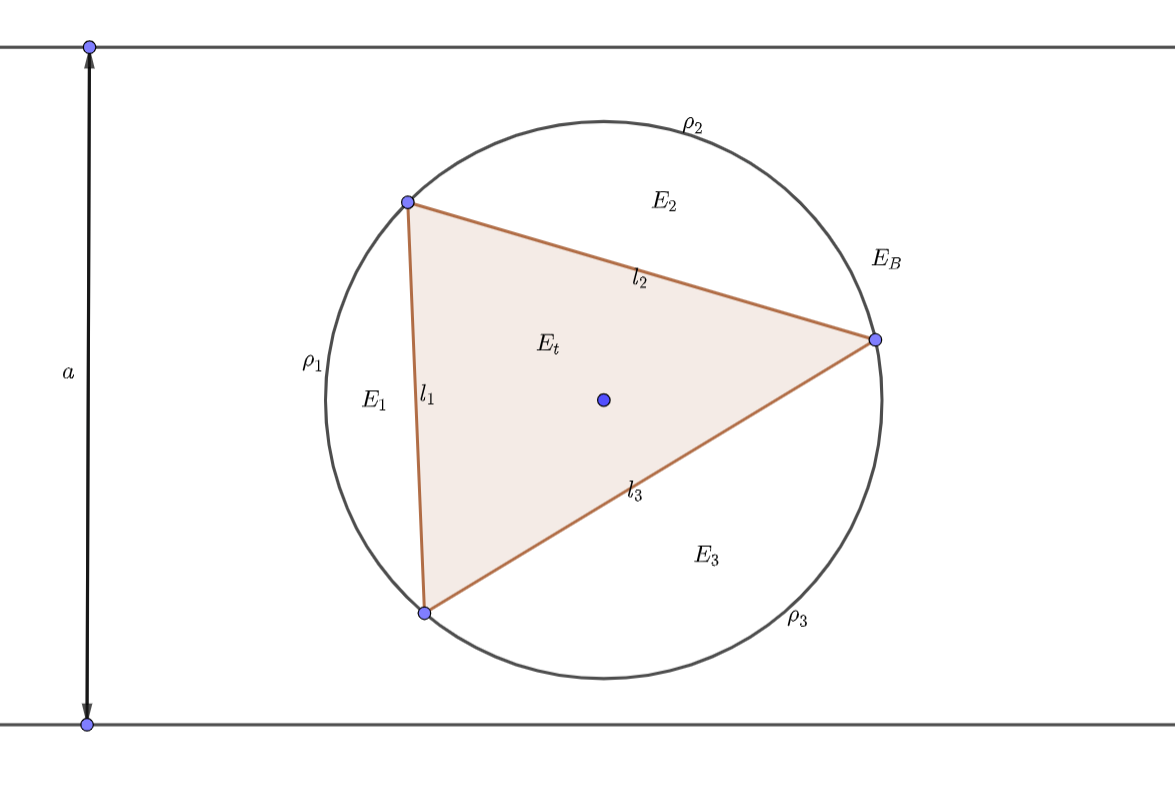
\includegraphics[width=0.8\textwidth]{figure.png}
}
% 表格模板
\renewcommand\arraystretch{0.8} % 设置表格高度为原来的0.8倍
\begin{table}[!htbp] % table标准
    \centering % 表格居中
    \begin{tabular}{p{1cm}<{\centering}p{1cm}<{\centering}p{3cm}<{\centering}p{5cm}<{\centering}} % 设置表格宽度
    %\begin{tabular}{cccc}
        \toprule
        $x_i$ & $f[x_1]$ & $f[x_i,x_{i+1}]$ & $f[x_i,x_{i+1},x_{i+2}]$ \\
        \midrule
        $x_0$ & $f(x_0)$ &                  &                          \\
        $x_0$ & $f(x_0)$ & $f'(x_0)$        &                          \\
        $x_0$ & $f(x_1)$ & $\frac{f(x_1)-f(x_0)}{x_1-x_0}$ & $\frac{f(x_1)-f(x_0)}{(x_1-x_0)^2}-\frac{f'(x_0)}{x_1-x_0}$\\
        \bottomrule
    \end{tabular}
\end{table}

\def\Log{\text{Log}} % 一个简单的宏定义
$\Log$ % 调用方法
\fi

\end{document}